\chapter{Érysichthon à jamais affamé}
\label{chap:erysichtonUsage}

intro


\section{Planification et préparations}

Nous avons nos spécificités technique et nous savons qu'elle forme notre outil doit avoir. Nous pouvons commencer par synthétiser les opérations nécessaires.\smallbreak

Nous allons donc concevoir des protocoles pour identifier les étapes nécessaires pour que Binsec analyse entièrement un fichier et nous renvoie un parmi [\texttt{secure, unknown, insecure}]. Le protocole \texttt{x86\_64} est particulier. Depuis la version \textbf{0.5.0} de Binsec il est possible de fournir un <<cliché mémoire>>\footnote{Plus couramment 'Core dump', terme technique anglais désignant une copie de la mémoire vive et des registres d'un programme. Ce fichier sert à être analyser, généralement par un débogueur.} pour accélérer l'analyse. On va se servir de cet avantage pour l'intégrer notre graphe d'éxécution.La machine sur laquelle le projet sera développé est sur une architecture x86\_64, cela nous permet d'utiliser l'outil GDB pour la génération de cliché mémoire.\medbreak

\begin{figure}[!ht]
    \caption{Protocole pour analyser des fichiers compiler en x86\_64}
    \label{fig:protocole_x86}
    \centering
  \begin{tikzpicture}[auto]

    % Styles
    \tikzstyle{startstop} = [rectangle, rounded corners, minimum width=2cm, minimum height=1cm, text centered, draw=black, fill=green!30]
    \tikzstyle{process} = [rectangle, minimum width=2cm, minimum height=1cm, text centered, draw=black, fill=orange!30]
    \tikzstyle{arrow} = [thick,->,>=stealth]
    \tikzset{zone1/.style={rectangle, rounded corners, draw=red, dashed, fill=red!10, inner sep=0.3cm}}
    \tikzset{zone2/.style={rectangle, rounded corners, draw=blue, dashed, fill=blue!10, inner sep=0.3cm, opacity = 0.7}}
    \tikzset{zone22/.style={rectangle, rounded corners, draw=none, fill=blue!10, inner sep=0.3cm}}
    \tikzset{zone3/.style={rectangle, rounded corners, draw=green, dashed, fill=green!10, inner sep=0.3cm}}
    
    % Noeuds
    \node (hacl) [startstop] {Hacl*};
    \node (c) [below of=hacl] {Fonction};
    \node (ini) [below of=c, xshift=2cm] {.ini};
    \node (test) [below of=c, xshift=-2cm] {-test.c};
    \node (script) [below of=c] {.script};
    \node (compilateur) [process, below of=test] {Compilateur};
    \node (exe) [below of=compilateur] {-test.exe};
    \node (blanc1) [below of=script] {};
    \node (blanc2) [below of=blanc1] {};
    \node (gdb) [process, below of=blanc2] {GDB};
    \node (snap) [right of=gdb, xshift=2cm] {.snapshot};
    \node (binsec) [startstop, right of=snap, xshift=1.5cm] {Binsec};
    
    % Flèches
    \draw [arrow] (hacl) -- (c);
    \draw [arrow] (c) -- (ini);
    \draw [arrow] (c) -- (test);
    \draw [arrow] (c) -- (script);
    \draw [arrow] (test) -- (compilateur);
    \draw [arrow] (compilateur) -- (exe);
    \draw [arrow] (exe) -- (gdb);
    \draw [arrow] (script) -- (gdb);
    \draw [arrow] (gdb) -- (snap);
    \draw [arrow] (snap) -- (binsec);
    \draw [arrow] (ini) -- (binsec);

    % Zones
    \begin{scope}[on background layer]
        \node [zone1, fit=(c) (ini) (test) (script)] {};
        \node [zone2, fit=(script) (gdb)] {};
              \node [zone2, fit=(gdb) (snap) (binsec)] {};
              \draw [zone22]
              ([xshift=-10pt, yshift=10pt]gdb.north west) --
              ([xshift=10pt, yshift=10pt]gdb.north east) -- 
              ([xshift=10pt, yshift=-9pt]gdb.south east) -- 
              ([xshift=1pt, yshift=-1pt]gdb.south west) --
              cycle;  
    \node [zone3, fit=(compilateur) (exe)] {};
    \end{scope}
    \end{tikzpicture}
\end{figure}

Ce graphe présente la chaîne d'étape à avoir pour obtenir une analyse Binsec depuis une fonction que l'on cible. Plusieurs zones sont distinguées. La zone verte correspond à l'étape de compilation, la zone bleue à l'étape de préparation de l'analyse et la zone rouge à la synthèse des fichiers de tests et d'instruction pour l'analyse. Ce choix de couleur est adapté à la difficulté attendu de chaque étape. L'opération de compilation consiste en une commande. L'opération de préparation d'analyse consiste aussi en deux commandes : un appel à GDB avec le binaire puis un appel à Binsec avec le cliché mémoire et les instruction d'analyse.\smallbreak

Avec ce graphe réalisé, on peut le modifier pour préparer la voie à d'autres architectures. Dans un format plus générique voici comment se présent notre protocole d'analyse :

\begin{figure}[!ht]
    \caption{Protocole générique d'analyse}
    \label{fig:protocole_generique}
    \centering
  \begin{tikzpicture}[auto]

    % Styles
    \tikzstyle{startstop} = [rectangle, rounded corners, minimum width=2cm, minimum height=1cm, text centered, draw=black, fill=green!30]
    \tikzstyle{process} = [rectangle, minimum width=2cm, minimum height=1cm, text centered, draw=black, fill=orange!30]
    \tikzstyle{arrow} = [thick,->,>=stealth]
    \tikzset{zone1/.style={rectangle, rounded corners, draw=red, dashed, fill=red!10, inner sep=0.3cm}}
    \tikzset{zone2/.style={rectangle, rounded corners, draw=blue, dashed, fill=blue!10, inner sep=0.3cm, opacity = 0.5}}
    \tikzset{zone3/.style={rectangle, rounded corners, draw=green, dashed, fill=green!10, inner sep=0.3cm}}
    
    % Noeuds
    \node (hacl) [startstop] {Hacl*};
    \node (c) [below of=hacl] {Fonction};
    \node (ini) [below of=c] {.ini};
    \node (test) [below of=c, xshift=-2cm] {-test.c};
    \node (compilateur) [process, below of=test] {Compilateur};
    \node (exe) [below of=compilateur] {-test.exe};
    \node (blanc) [below of=c] {};
    \node (blanc1) [below of=blanc] {};
    \node (blanc2) [below of=blanc1] {};
    \node (binsec) [startstop, below of=blanc2] {Binsec};
    
    % Flèches
    \draw [arrow] (hacl) -- (c);
    \draw [arrow] (c) -- (ini);
    \draw [arrow] (c) -- (test);
    \draw [arrow] (test) -- (compilateur);
    \draw [arrow] (compilateur) -- (exe);
    \draw [arrow] (exe) -- (binsec);
    \draw [arrow] (ini) -- (binsec);

    % Zones
    \begin{scope}[on background layer]
        \node [zone1, fit=(c) (ini) (test) ] {};
        \node [zone2, fit=(ini) (binsec)] {};
        \node [zone3, fit=(compilateur) (exe)] {};
    \end{scope}    
    \end{tikzpicture}
\end{figure}

Dans ce contexte, une question se pose : est-ce que la conception des script pour Binsec (\textit{.ini}) est automatisable ou est-ce qu'il faudra utiliser des émulateurs pour générer des clichés mémoire et revenir dans le cas de la figure \ref{fig:protocole_x86} ?\smallbreak

Cette question est importante parce que lorsqu'on analyse un fichier ARM par exemple, si le fichier source contient des appels à des fonctions systèmes, les \texttt{IFUNC}, celles-ci sont exécutées en fonction de l'architecture qui exécute le programme. Or Binsec n'a pas ces informations, il faut les fournir à la main. Voici le scipt nécessaire pour une vérification de la fonction <<Hacl \_AEAD \_Chacha20Poly1305\_Simd128\_encrypt>> compilé vers ARMv8.

\begin{listing}[!ht]
    \caption{Script d'instruction pour analyser un binaire compilé vers ARM}
    \label{lst:script_arm_exemple}
    \begin{minted}{bash}
load sections .plt, .text, .rodata, .data, .got, .got.plt, .bss from file

secret global input1, aad1

@[0x00000048f008 ,8] := <__memcpy_generic>
@[0x00000048f018, 8] := <__memset_generic>
@[0x00000048f030 ,8] := <__memcpy_thunderx2>

lr<64> := 0xdeadbeef as return_address

starting from <main>
with concrete stack pointer

halt at return_address
halt at <_IO_puts>
explore all 
    \end{minted}
\end{listing}

Les lignes 5 à 7 sont présente pour indiquer les branchement à effectuer par Binsec lorsque qu'il rencontre ces adresses. Cette opération automatiquement exécutée lors de l'initialisation de l'exécution doit ici être précisée avec les fonction présente dans le binaire. Automatiser ces affectations peut être difficile et nécessiter quelques outils d'analyse supplémentaires pour attraper les adresses qui ont besoin d'être réaffecté et leur attribuer les fonctions les plus adaptées.\medbreak


\begin{CitationBox}{Nommer un outil}
    Rapidement il a fallu trouver un nom pour ce projet, l'appeler par "Notre outil\dots" devenait lourd et redondant entre les réunion hebdomadaire. En revanche trouver LE nom adéquat n'est pas une chose aisée, il peut être dû à une blague, une référence ou plus simplement liés au sens du projet. Dans notre cas, on aime la mythologie et le travail réalisé peut se résumer à "faut donner à manger à Binsec".\smallbreak
    Érysichthon est une personnage de la mythologie grecque condamné à être affamé au point de se dévorer lui-même pour avoir détruit l'idole d'un dieu. Ce nom me plaît et sera retenu pour la suite du projet. 
\end{CitationBox}

\subsection*{Conception d'Érysichthon}

On a des protocoles. On a des expériences sur des fonctions de Hacl*. On a un nom. Il faut maintenant passer à l'échelle et concevoir un outil complet qui intéragit et exécute nos instructions. L'outil sera en somme une combinaison de script python, shell et de Makefile. Il faut donc les organiser et adapter leurs intéractions pour arriver au bout de nos peines.

\begin{figure}[!ht]
    \caption{Structure des modules d'Érysichthon}
    \label{fig:erysichton}
    \centering
    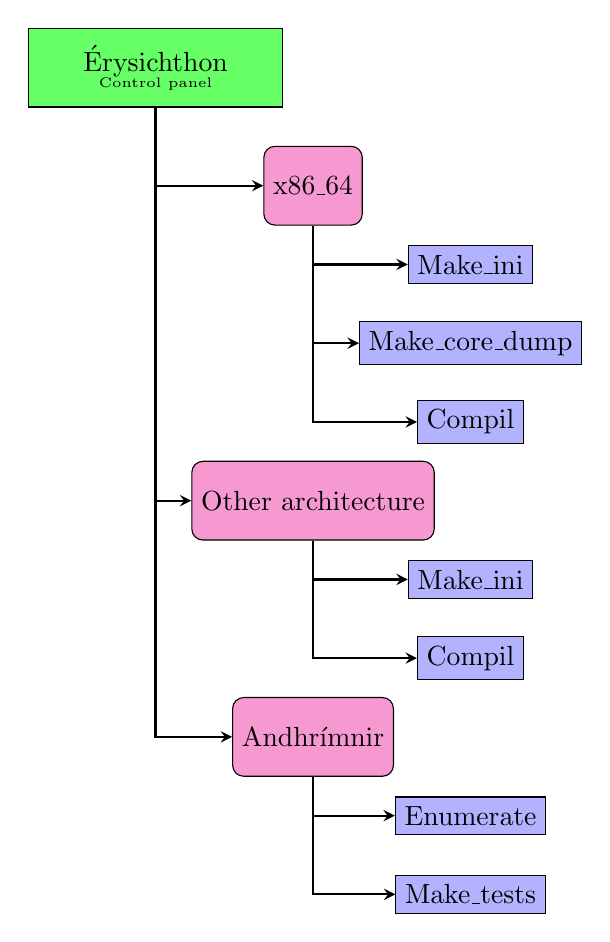
\begin{tikzpicture}[auto]

    % Styles
    \tikzstyle{startstop} = [rectangle, minimum width=2cm, minimum height=1cm, text centered, draw=black, fill=green!60]
    \tikzstyle{process} = [rectangle, rounded corners,minimum width=1cm, minimum height=1cm, text centered, draw=black, fill=magenta!40]
     \tikzstyle{process2} = [rectangle, minimum width=0.8cm, minimum height=0.3cm, text centered, draw=black, fill=blue!30]
    \tikzstyle{arrow} = [thick,->,>=stealth]
    
    % Noeuds
    \node (control) [startstop] {\parbox{3cm}{\centering Érysichthon \\ \tiny{Control panel}}};
    \node (x86) [process, below of=control, xshift= 2cm, yshift=-0.5cm] {x86\_64};
    \node (x86-ini) [process2, below of=x86, xshift = 2cm] {Make\_ini};
    \node (x86-dump) [process2, below of=x86-ini] {Make\_core\_dump};
    \node (x86-compil) [process2, below of=x86-dump] {Compil};
    \node (arm) [process, below of=x86-compil, xshift=-2cm] {Other architecture};
    \node (arm-ini) [process2, below of=arm, xshift=2cm] {Make\_ini};
    \node (arm-compil) [process2, below of=arm-ini] {Compil};
    \node (test) [process, below of=arm-compil, xshift=-2cm] {Andhrímnir};
    \node (enum) [process2, below of=test, xshift=2cm] {Enumerate};
    \node (exe) [process2, below of=enum] {Make\_tests};

    % Flèches
    \draw [arrow] (control) -- ++(0,-1.5) -- (x86);
    \draw [arrow] (control) -- ++(0,-5.5) -- (arm);
    \draw [arrow] (control) -- ++(0,-8.5) -- (test);
    \draw [arrow] (x86) -- ++(0,-1) -- (x86-ini);
    \draw [arrow] (x86) -- ++(0,-2) -- (x86-dump);
    \draw [arrow] (x86) -- ++(0,-3) -- (x86-compil);
    \draw [arrow] (arm) -- ++(0,-1) -- (arm-ini);
    \draw [arrow] (arm) -- ++(0,-2) -- (arm-compil);
    \draw [arrow] (test) -- ++(0,-1) -- (enum);
    \draw [arrow] (test) -- ++(0,-2) -- (exe);
    
    \end{tikzpicture}
\end{figure}

On retrouve les différentes étapes de nos protocoles représentées par des modules au sein de leur noeuds respectifs : <<\texttt{Make\_ini}>> pour les scripts pour Binsec, <<\texttt{Make\_core\_dump}>> pour la génération des clichés mémoires et <<\texttt{Compil}>> pour les appels aux compilateurs. Le dernier noeud <<\texttt{Andhrímnir}>> est particulier et détaillé dans la section suivante. 

\subsection*{Andhrímnir}

Ce module de Érysichthon est particulier. Premièrement c'est le seul qui est aussi son nom. Ce module consiste a produire les fichiers qui seront compilés puis analysés par Binsec. Ce module est nommé d'après le cuisinier de la mythologie nordique, car comme lui, il prépare sempiternellement des mets pour son maître.\smallbreak

Ce module est nommé car il constitue un projet dans le projet, sa seule conception pris plus de la moitié du temps de développement total. C'est un outil qui, à partir d'un projet en C, est capable de générer automatiquement des tests qui compilent et peuvent ensuite être proposé à des outils d'analyse binaire. Ce module est aggrégé à Érysichthon mais peut être porter vers d'autre projets. À la différence des logiciels qui produisent des tests unitaires ( uniquement sur des projet Java, Haskell ou C\# et souvent associé à des offres payantes), on a ici une couverture complète des fonctions portés par le projet C.\smallbreak

Ce module, comme son grand frère, fonctionne et est abouti, par contre il nécessite quelques opérations manuelles et peut être améliorer pour pouvoir supporter d'autre projet C. Actuellement il possède quelques optimisation associées à Hacl* pour accélérer la réalisation de la preuve de concept.

\section{Conception et usages}

On va commencer par le petit frère, Andhrímnir. Il fonctionne avec une phase d'initialisation <<\texttt{Enumerate}>> et une phase de production de tests <<\texttt{Make\_tests}>>, elle même découpé en plusieurs étapes. La génération de \textbf{548} fichiers de tests est réalisé moins de 2 secondes.\smallbreak

\subsection*{Enumerate}

Cette étape, de réalisation très simple, consiste à identifier toutes les fonctions qui auront un fichier test généré. Comme Hacl* génère automatiquement son code C, on peut exploiter cette particularité pour lister rapidement nos fonctions. L'opération actuellement réalisé est de lister l'ensemble des fichiers "\textbf{.h}" contenu dans le répertoire cible. Ensuite un parcours et une lecture de ceux-ci nous donne toutes les fonctions de l'API d'Hacl* et d'avoir une couverture complète du projet.\smallbreak

C'est lors de cette étape que l'on peut spécifier ou retirer des fichiers ou plus précisément des fonctions de la chaîne de production. Ce garde fou permet d'accélérer l'obtention des résultats finaux et d'aider grandement lorsque l'on souhaite débuguer.

\subsection*{Make\_test}


\begin{figure}
    \caption{Schéma de conception d'Andhrímnir}
    \label{fig:schema_andrhimnir}
    \centering
    \begin{tikzpicture}[auto]
    % Définition des styles pour les boîtes et flèches
    \tikzset{
      box1/.style={rectangle, draw=black, fill=cyan!30, thick, rounded corners, minimum width=2.5cm, minimum height=1cm, align=center},
      box2/.style={rectangle, draw=black, fill=orange!30, thick, rounded corners, minimum width=2.5cm, minimum height=1cm, align=center},
      box3/.style={rectangle, draw=black, fill=yellow!30, thick, rounded corners, minimum width=2.5cm, minimum height=1cm, align=center},
      box4/.style={rectangle, draw=black, fill=green!30, thick, rounded corners, minimum width=2.5cm, minimum height=1cm, align=center},
      box5/.style={rectangle, draw=black, fill=blue!30, thick, rounded corners, minimum width=2.5cm, minimum height=1cm, align=center},
      box6/.style={rectangle, draw=black, fill=magenta!30, thick, rounded corners, minimum width=2.5cm, minimum height=1cm, align=center},
      box65/.style={rectangle, draw=black, fill=magenta!60, thick, rounded corners, minimum width=1.5cm, minimum height=0.6cm, align=center},
      box7/.style={rectangle, draw=black, fill=red!30, thick, rounded corners, minimum width=2.5cm, minimum height=1cm, align=center},
      box8/.style={rectangle, draw=black, fill=blue!45, thick, rounded corners, minimum width=2.5cm, minimum height=1cm, align=center},
      arrow1/.style={->, thick, color=cyan!70!black},
      arrow2/.style={->, thick, color=orange!80!black},
      arrow3/.style={->, thick, color=yellow!80!black},
      arrow4/.style={->, thick, color=green!80!black},
      arrow5/.style={->, thick, color=blue!80!black},
      arrow6/.style={->, thick, color=magenta!80!black},
      arrow7/.style={->, thick, color=red!80!black},
      arrow8/.style={->, thick, color=gray!80!black}
    }

    % Noeuds principaux (ligne du haut)
    \node[box1] (build_test) at (0,0) {build\_test};
    \node[box2, below of=build_test, yshift=-0.3cm] (parse_h) {Lecture du .h};
    \node[box3, right=1cm of parse_h] (read_json) {Lecture json générique};
    \node[box4, right=1cm of read_json] (build_local_json) {Capture des informations};

    % Ligne du bas (génération du .c)
    \node[box5, below=1cm of build_local_json] (build_intro) {Gen. introduction};
    \node[box6, left=1cm of build_intro] (build_def) {Gen. definition};
    \node[box7, left=1cm of build_def] (add_main) {Gen. main};
    \node[box8, left=1cm of add_main] (fichier_c) {fichier .c};

    % Flèches horizontales principales
    \draw[arrow1] (build_test) -- (parse_h);
    \draw[arrow2] (parse_h) -- (read_json);
    \draw[arrow3] (read_json) -- (build_local_json);
    \draw[arrow4] (build_local_json) -- (build_intro);
    \draw[arrow5] (build_intro) -- (build_def);
    \draw[arrow6] (build_def) -- (add_main);
    \draw[arrow7] (add_main) -- (fichier_c);

    % Branche auxiliaire depuis build introduction
    \node[box5, left of = build_intro, yshift=-1cm] (detect_aux) {Détection appel auxiliaire};
    % Ajout de deux barres obliques sur la flèche build_intro -> build_def
    \draw[thick] ($(build_intro)!0.5!(build_def) + (0,0.3)$) -- ($(build_intro)!0.5!(build_def) + (0,-0.54)$);
    \draw[thick] ($(build_intro)!0.55!(build_def) + (0,0.3)$) -- ($(build_intro)!0.55!(build_def) + (0,-0.54)$);


    \node[box3, left=1cm of detect_aux, yshift=-1cm] (test_exist) {test si fichier existe};
    \draw[arrow5] (detect_aux) -- (test_exist);

    % Oui -> Collage -> build definition
    \node[box65, above of = test_exist] (collage) {\footnotesize{Collage}};
    \draw[->, thick, color=green!80!black] (test_exist) -- node[font=\scriptsize] {Oui} (collage);
    \draw[arrow6] (collage) -- (build_def);

    % Non -> Stocker dans liste_temporisée
    \node[box8, left=0.8cm of test_exist, yshift=-0.8cm] (liste_temp) {Stocker dans liste\_temporisée};
    \draw[arrow7] (test_exist) -- node[font=\scriptsize] {Non} (liste_temp);
  \end{tikzpicture}
\end{figure}


\vfill
\textit{Transition}